\begin{enumerate}[label=\thesubsection.\arabic*,ref=\thesubsection.\theenumi]
    \item Find the shortest distance between the lines whose vector equations are
    \begin{align}
        \vec{x} = \myvec{1\\2\\3} + \lambda_1\myvec{1\\-3\\2}
    \end{align}
    and
    \begin{align}
        \vec{x} = \myvec{4\\5\\6} + \lambda_2\myvec{2\\3\\1}
    \end{align}
    \solution
		\\ \solution 
\begin{align}
    \vec{A}-\vec{F}&=\myvec{1\\-1}-\myvec{\frac{-3}{2}\\\frac{5}{2}}
    =\myvec{\frac{5}{2}\\\frac{-7}{2}}
    \\
    \vec{E}-\vec{D}&=\myvec{-1\\-3}-\myvec{\frac{-7}{2}\\\frac{1}{2}}
    =\myvec{\frac{5}{2}\\\frac{-7}{2}}
    \\
	\implies	\vec{A}-\vec{F} &= \vec{E}-\vec{D}
\end{align}
See \figref{fig:Triangle-pgm}, 
\begin{figure}
\centering
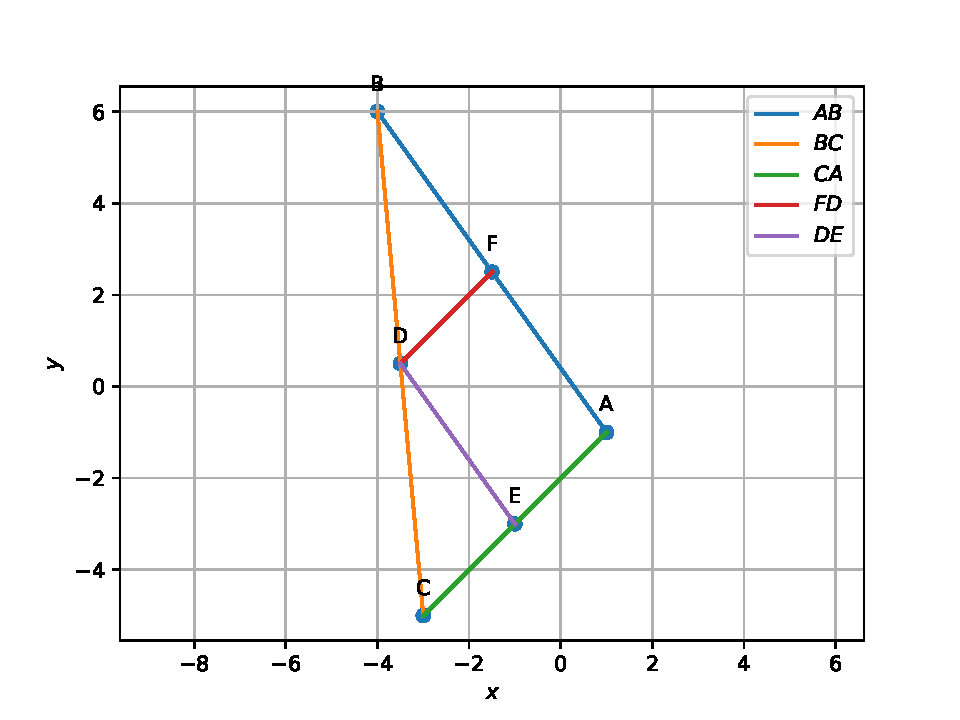
\includegraphics[width=0.75\columnwidth]{figs/triangle/pgm.pdf}
\caption{$AFDE$ forms a parallelogram in triangle ABC}
\label{fig:Triangle-pgm}
\end{figure}






















\item Find the shortest distance between the lines $l_1$ and $l_2$ whose vector equations are 
\begin{align}
	\overrightarrow{r} &= \hat{i}+\hat{j}+\lambda(2\hat{i}-\hat{j}+\hat{k}) \text{ and}
	\\
	\overrightarrow{r} &= 2\hat{i}+\hat{j}-\hat{k}+\mu(3\hat{i}-5\hat{j}+2\hat{k}).
\end{align}
    \solution
		\\ \solution 
\begin{align}
    \vec{A}-\vec{F}&=\myvec{1\\-1}-\myvec{\frac{-3}{2}\\\frac{5}{2}}
    =\myvec{\frac{5}{2}\\\frac{-7}{2}}
    \\
    \vec{E}-\vec{D}&=\myvec{-1\\-3}-\myvec{\frac{-7}{2}\\\frac{1}{2}}
    =\myvec{\frac{5}{2}\\\frac{-7}{2}}
    \\
	\implies	\vec{A}-\vec{F} &= \vec{E}-\vec{D}
\end{align}
See \figref{fig:Triangle-pgm}, 
\begin{figure}
\centering
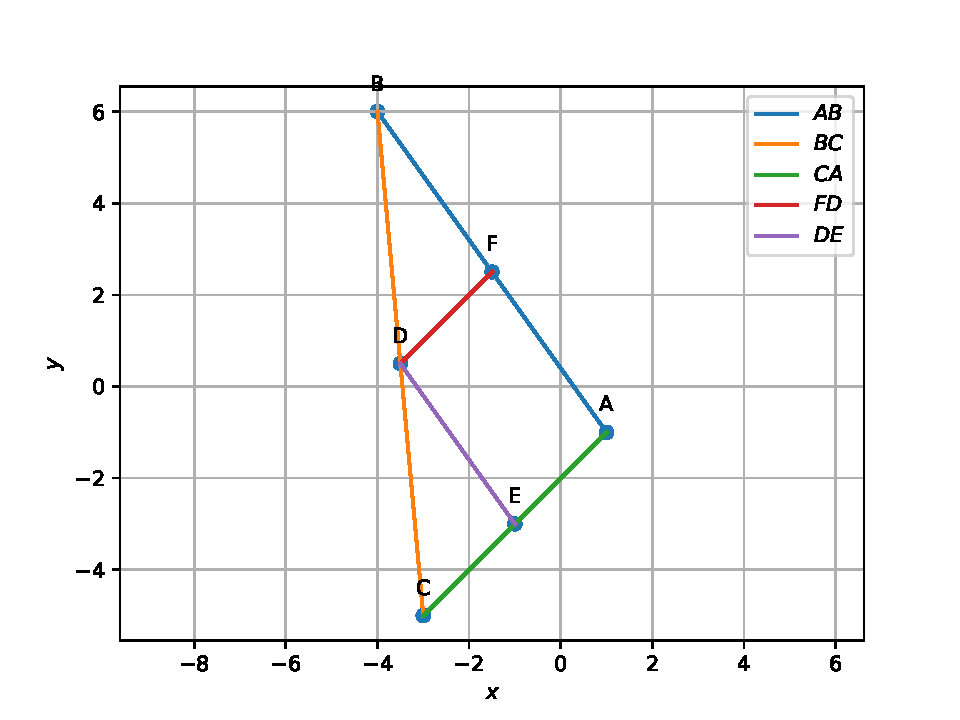
\includegraphics[width=0.75\columnwidth]{figs/triangle/pgm.pdf}
\caption{$AFDE$ forms a parallelogram in triangle ABC}
\label{fig:Triangle-pgm}
\end{figure}






















\item Find the shortest distance between the lines given by 
\begin{align}
	\overrightarrow{r}&=(8+3\lambda\hat{i}-(9+16\lambda)\hat{j}+(10+7\lambda)\hat{k} \text{ and} 
	\\
	\overrightarrow{r}&=15\hat{i}+29\hat{j}+5\hat{k}+\mu(3\hat{i}+8\hat{j}-5\hat{k}).
\end{align}
\item Find the shortest distance between the lines
\begin{align}
	\overrightarrow{r}&=(\hat{i}+2\hat{j}+\hat{k})+\lambda(\hat{i}-\hat{j}+\hat{k}) \text{ and} 
	\\
	\overrightarrow{r}&=2\hat{i}-\hat{j}-\hat{k}+\mu(2\hat{i}+\hat{j}+2\hat{k})
\end{align}
\item Find the shortest distance between the lines
\begin{align}
	\frac{x+1}{7}&=\frac{y+1}{-6}=\frac{z+1}{1} \text{ and}
	\\
	\frac{x-3}{1}&=\frac{y-5}{-2}=\frac{z-7}{1}
\end{align}
\end{enumerate}
